\section{سوال اول}
این مسئله با دو روش رمزنگاری\LTRfootnote{encoding}
ژن‌ها انجام شده است. روش اول، روش اشاره شده در صورت سوال است و روش دوم رمزنگاری به صورت دودویی\LTRfootnote{binary}
 است. این دو روش نیز در انتها با تابع \lr{ga}
 برنامه
 \lr{MATLAB}
 مقایسه شده است.

کروموزم تولید شده در ماتریس پایین آورده شده است.
$$
\begin{bmatrix}
	4 & 3 & 6 & 2 & 3 & 2 & 3 & 4 & 4 & 0 & 7 & 1 & 3 & 4 
\end{bmatrix}
$$
\begin{figure}[H]
 	\caption{کروموزوم یک جواب تولید شده به صورت تصادفی} 
 	\vspace{-3cm}
 	\centering 
 	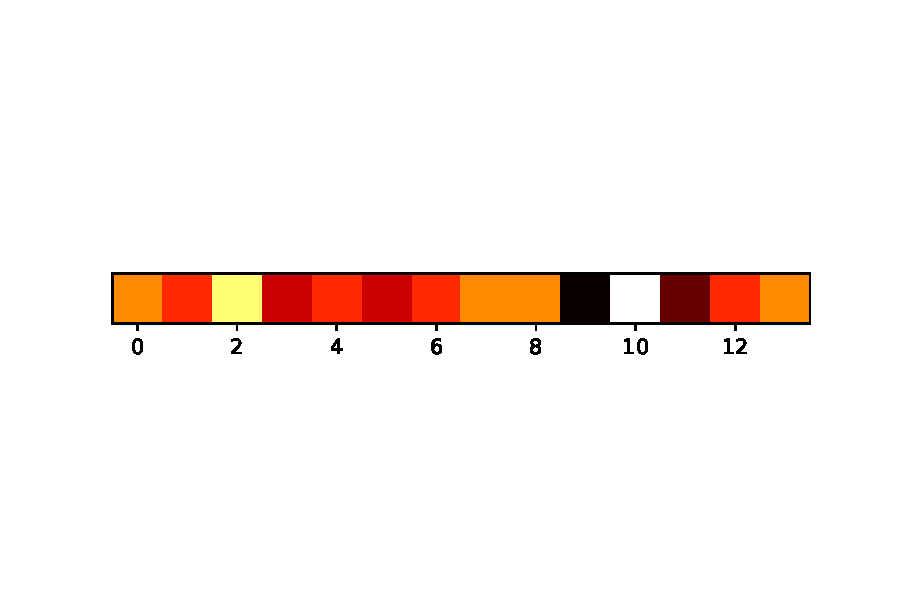
\includegraphics[width=12cm]{../Figure/Q1/chromosome0} 
 \end{figure}
\vspace{-3cm}
\begin{figure}[H]
	\caption{جواب کروموزوم یک جواب تولید شده به صورت تصادفی} 
	\centering 
	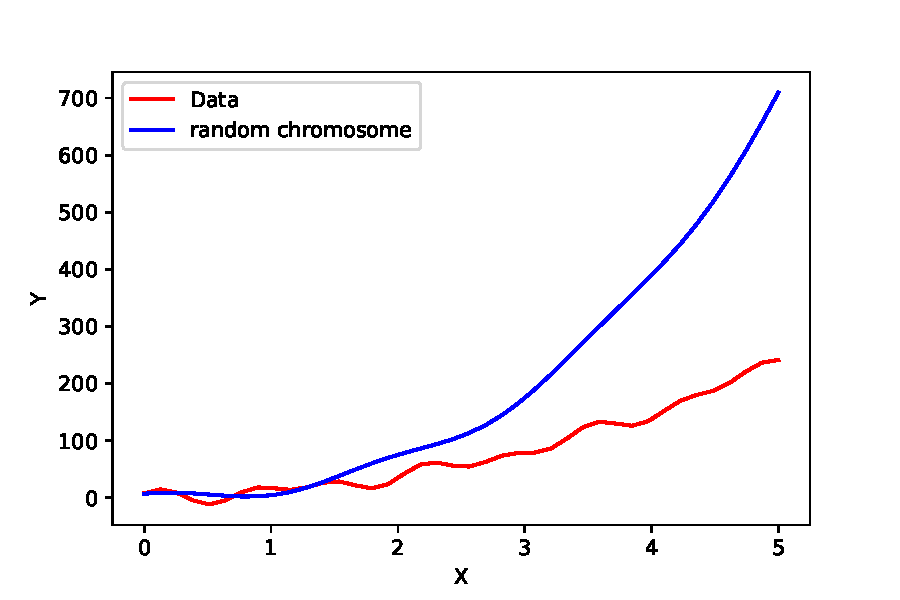
\includegraphics[width=12cm]{../Figure/Q1/ans0} 
\end{figure}

\begin{figure}[H]
	\caption{کروموزوم یک جواب تولید شده به صورت تصادفی و دودویی} 
		\vspace{-3cm}
	\centering 
	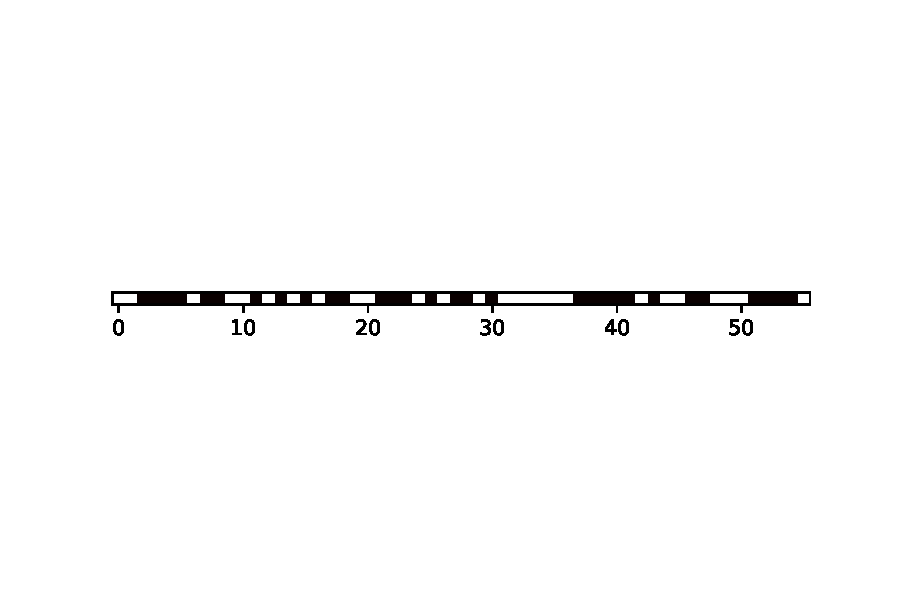
\includegraphics[width=12cm]{../Figure/Q1/chromosome1} 
\end{figure}
\vspace{-3cm}
\begin{figure}[H]
	\caption{جواب کروموزوم یک جواب تولید شده به صورت تصادفی و دودویی} 
	\centering 
	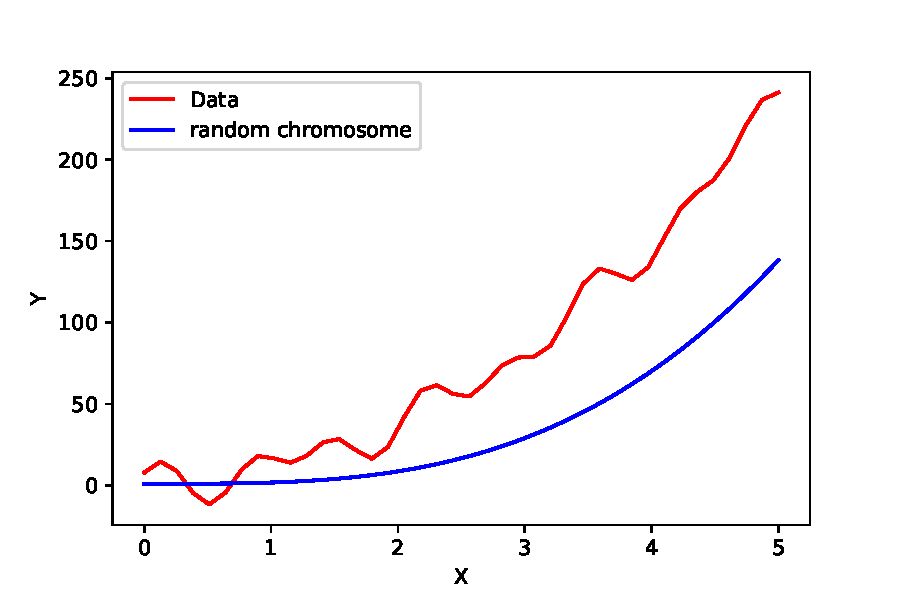
\includegraphics[width=12cm]{../Figure/Q1/ans1} 
\end{figure}

\begin{figure}[H]
	\caption{کروموزوم دو والد تولید شده به صورت تصادفی} 
	\vspace{-3cm}
	\centering 
	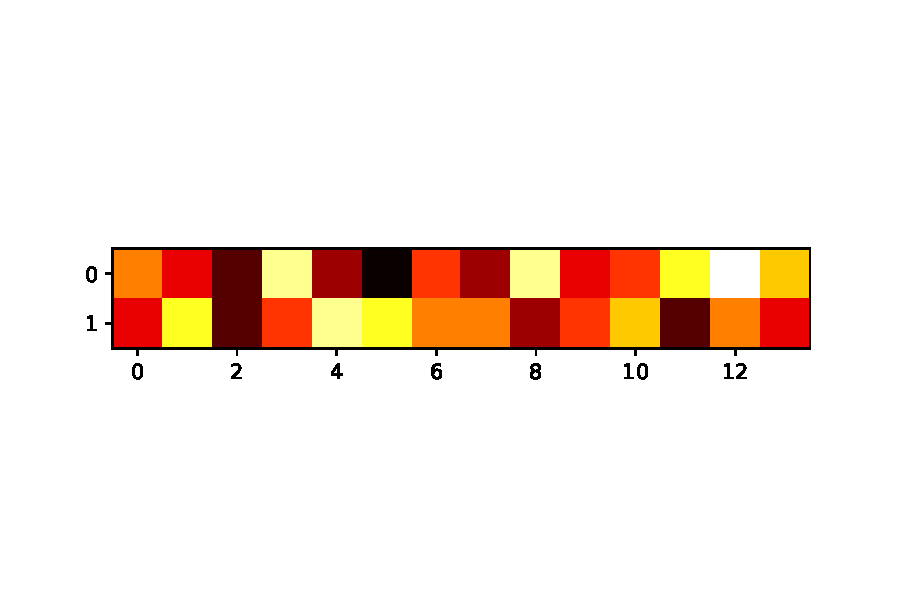
\includegraphics[width=12cm]{../Figure/Q1/parent} 
\end{figure}
\vspace{-3cm}
\begin{figure}[H]
	\caption{کروموزوم دو فرزند تولید شده از والد اشاره شده به صورت \lr{One Point Cross-over}} 
	\vspace{-3cm}
	\centering 
	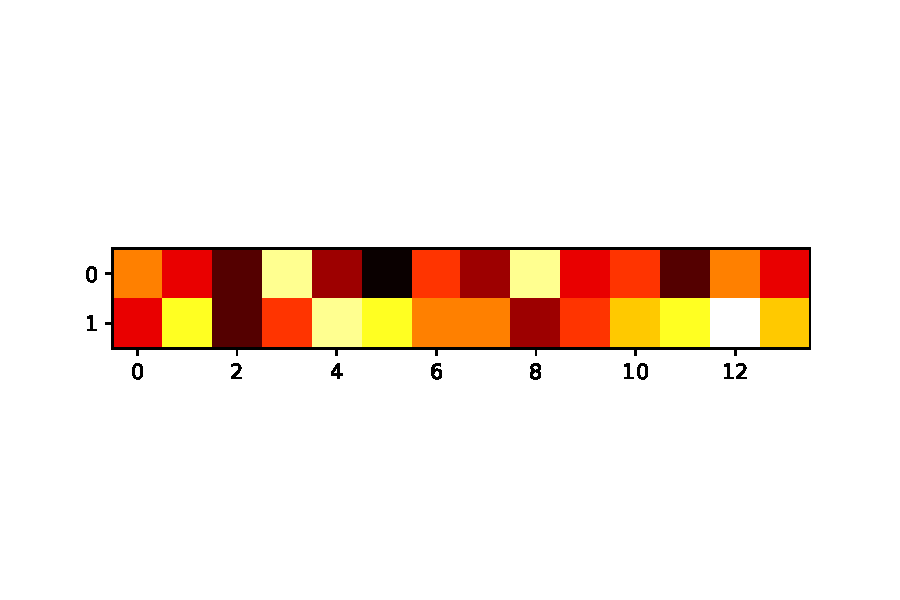
\includegraphics[width=12cm]{../Figure/Q1/child} 
\end{figure}

\vspace{-3cm}
\begin{figure}[H]
	\caption{کروموزوم والد و فرزندان} 
	\vspace{-2cm}
	\centering 
	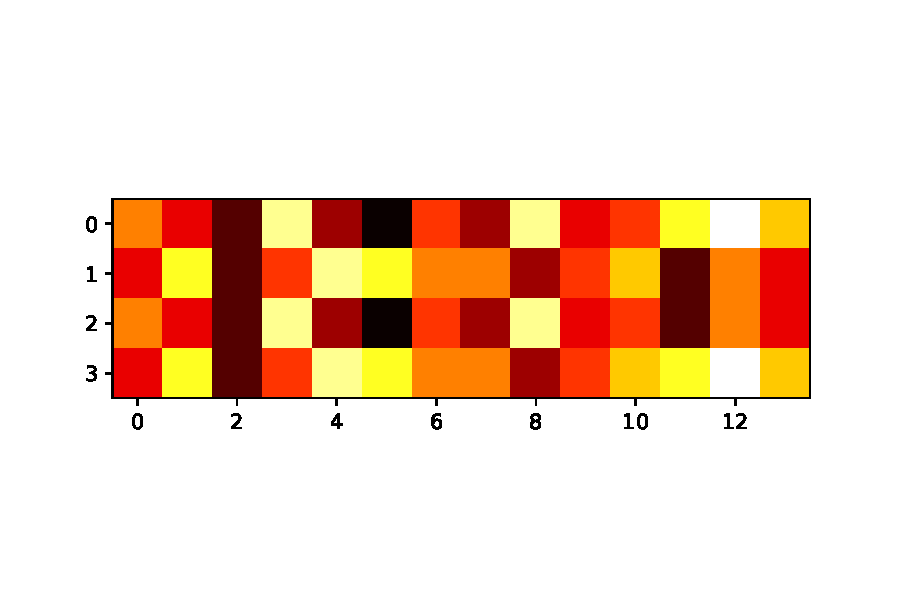
\includegraphics[width=12cm]{../Figure/Q1/all} 
\end{figure}
\vspace{-2cm}


\begin{figure}[H]
	\caption{کروموزوم دو والد تولید شده به صورت تصادفی و دودویی} 
	\vspace{-3.5cm}
	\centering 
	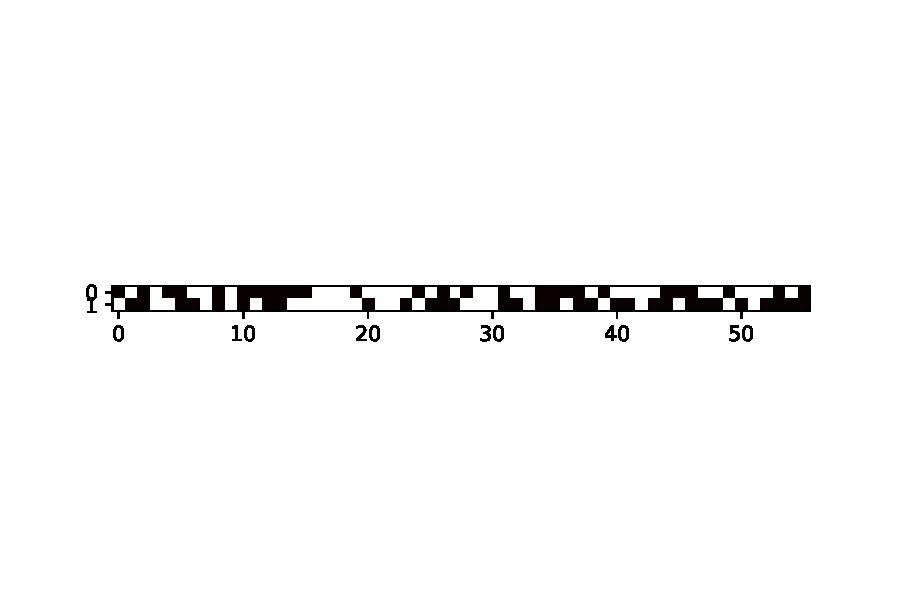
\includegraphics[width=12cm]{../Figure/Q1/parent_ba} 
\end{figure}
\vspace{-3.5cm}
\begin{figure}[H]
	\caption{کروموزوم دو فرزند تولید شده از والد اشاره شده به صورت \lr{Uniform crossover}} 
	\vspace{-3.5cm}
	\centering 
	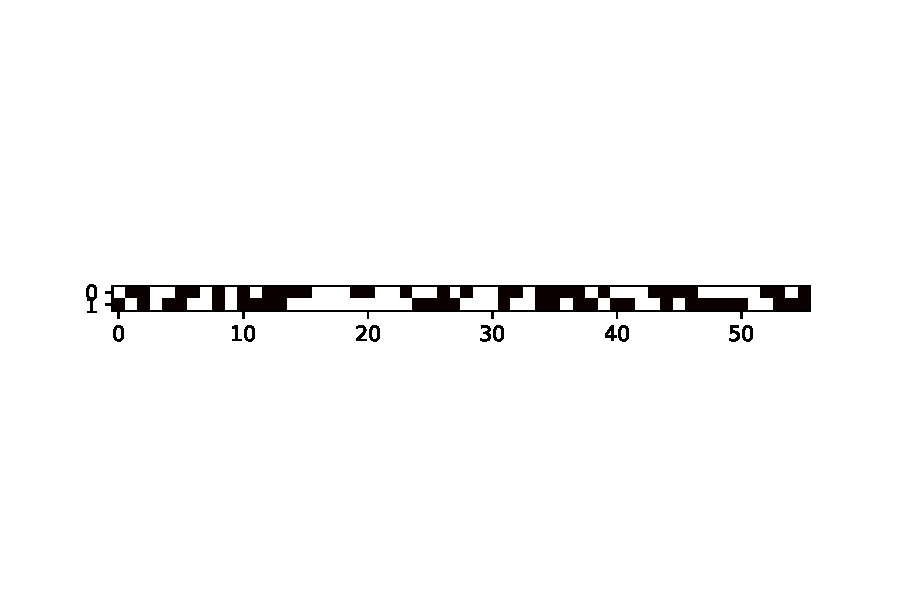
\includegraphics[width=12cm]{../Figure/Q1/child_ba} 
\end{figure}

\vspace{-3.5cm}
\begin{figure}[H]
	\caption{کروموزوم والد و فرزندان به صورت دودویی} 
	\vspace{-3.5cm}
	\centering 
	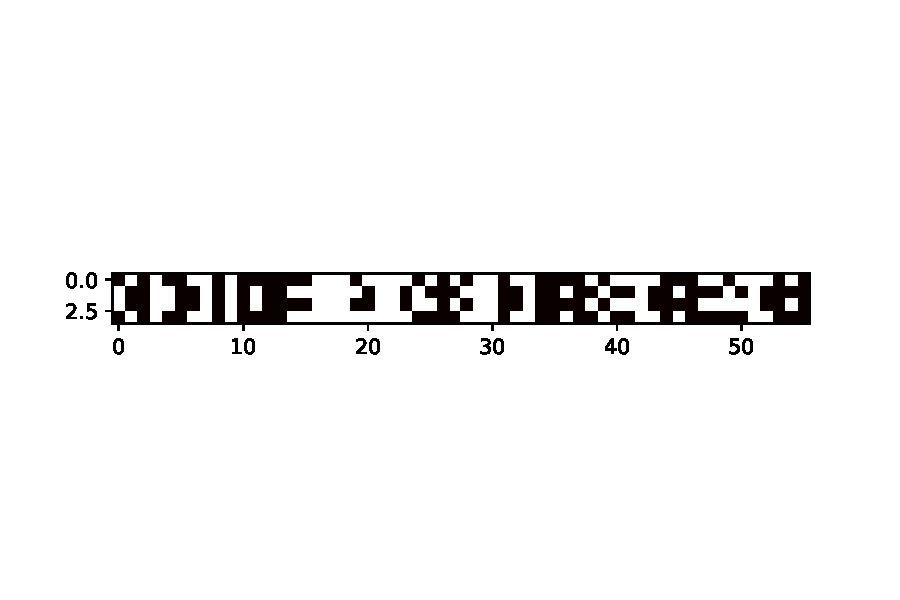
\includegraphics[width=12cm]{../Figure/Q1/all_ba} 
\end{figure}
\vspace{-3.5cm}
فرایند جهش به این صورت است که، اگر عدد تصادفی تولید شده از ضریب جهش کمتر باشد، یک ژن به صورت تصادفی انتخاب می‌شود و یک عدد تصادفی جایگزین آن می‌شود.
\begin{figure}[H]
	\caption{کروموزوم قبل و بعد از جهش} 
	\vspace{-3cm}
	\centering 
	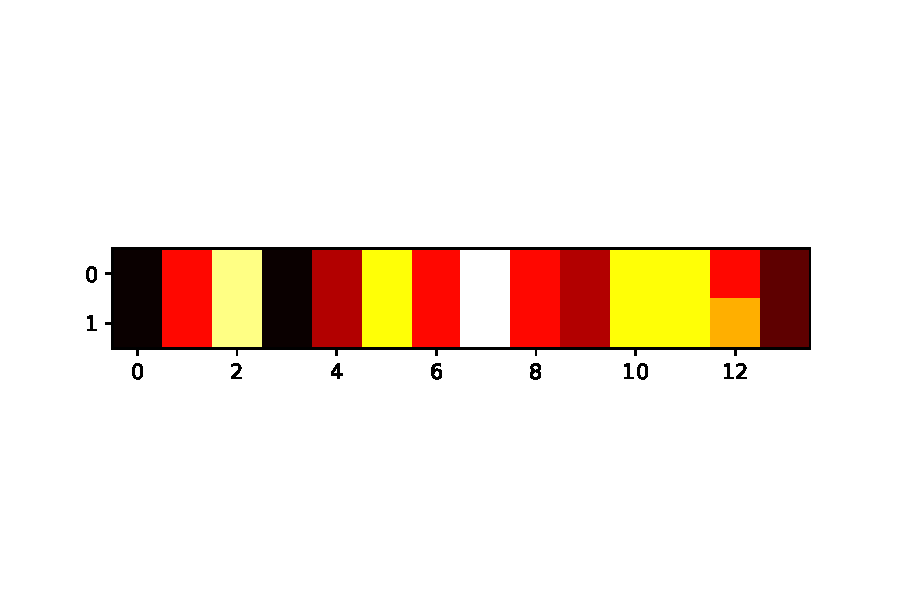
\includegraphics[width=12cm]{../Figure/Q1/all_mutate} 
\end{figure}
\vspace{-3cm}
در مرحله انتخاب، از روش
\lr{Double Tournament Selection}
استفاده شده است. برای انتخاب والد و جایگزین دو
\lr{tournament}
برگذار می‌شود. در هر
\lr{tournament}
کرموزوم‌ها بر اساس تابع هزینه مرتب می‌شود و بر اساس تابع هزینه یا معکوس تابع هزینه (بستگی به انتخاب والد و یا جایگزین دارد) احتمال انتخاب افراد مشخص می‌شود. در ادامه اگر شخصی که برای جایگزینی انتخاب شد نفر اول باشد (کمترین تابع هزینه را داشته باشد) عملیات جایگزینی انجام نمی‌شود تا نخبه‌گرایی رعایت شود. پارامتر‌های آن سایز 
\lr{tournament}
و تعداد جمعیت است.

پارامترهای الگوریتم ژنتیک نوشته شده شامل جمعیت، ضریب احتمال انجام
\lr{cross-over}،
ضریب احتمال انجام
\lr{mutation}،
سایز
\lr{tournament}
و تعداد نسل‌ها است که به صورت
\lr{greedy}
انتخاب شده است.

\begin{figure}[H]
	\caption{تابع هزینه بر حسب شماره نسل} 
	\centering 
	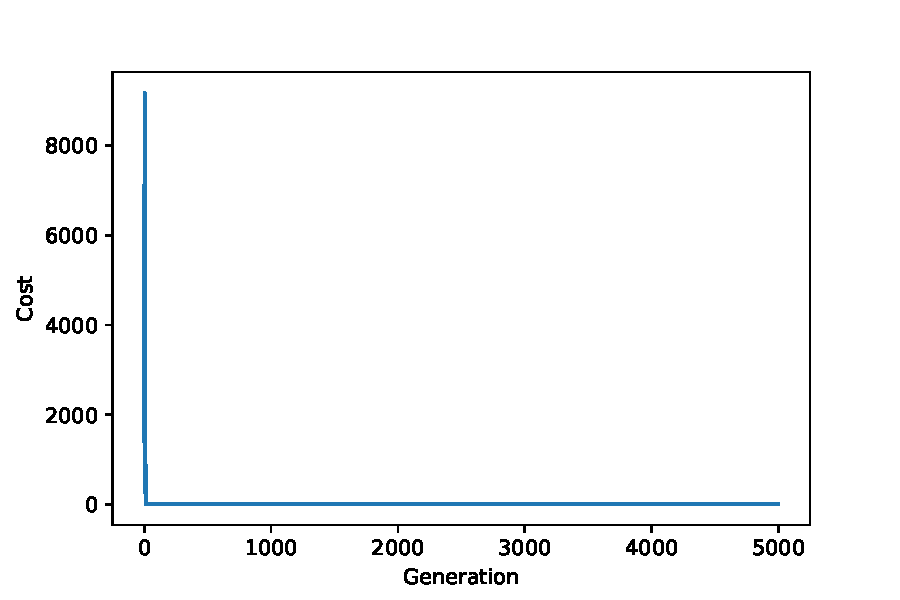
\includegraphics[width=12cm]{../Figure/Q1/history} 
\end{figure}

 نتایج جدول‌ها بر اساس ده بار اجرا کد با شرایط نوشته شده است.
 	\lr{\begin{table}[H]
		 			\caption{cross-over rate study}
		 			\vspace{0.5cm}
		 			\centering
		 			\begin{tabular}{|c|c|c|c|}
			 				\hline
			 				 Min & \lr{Standard deviation} & Mean & \lr{cross-over rate}  \\
			 				\hline 
			 				20.89 & 4847.33 & 363.26 & 0.9 \\
			 				6.57 & 404.02 & 221.08 & 0.5 \\
			 				42.33 & 493.30 & 517.17 & 0.1 \\
			 				\hline
			 			\end{tabular}
\end{table}}

 	\lr{\begin{table}[H]
		\caption{mutation rate study}
		\vspace{0.5cm}
		\centering
		\begin{tabular}{|c|c|c|c|}
			\hline
			Min & \lr{Standard deviation} & Mean & \lr{mutation rate}  \\
			\hline 
			20.89 & 4847.33 & 363.26 & 0.5 \\
			48.38  & 643.18 & 779.47 & 0.1 \\
			1593.25  & 255.48 & 2108.53 & 0.05 \\
			\hline
		\end{tabular}
\end{table}}

 	\lr{\begin{table}[H]
		\caption{population}
		\vspace{0.5cm}
		\centering
		\begin{tabular}{|c|c|c|c|}
			\hline
			Min & \lr{Standard deviation} & Mean & \lr{population}  \\
			\hline 
			20.89 & 4847.33 & 363.26 & 100 \\
			13.80 & 1010.17 & 823.29& 50 \\
			15.20 & 493.87 & 459.00 & 20 \\
			\hline
		\end{tabular}
\end{table}}

\begin{figure}[H]
	\caption{جواب الگوریتم ژنتیک بر اساس پارامترهای تنظیم شده به صورت \lr{greedy}} 
	\centering 
	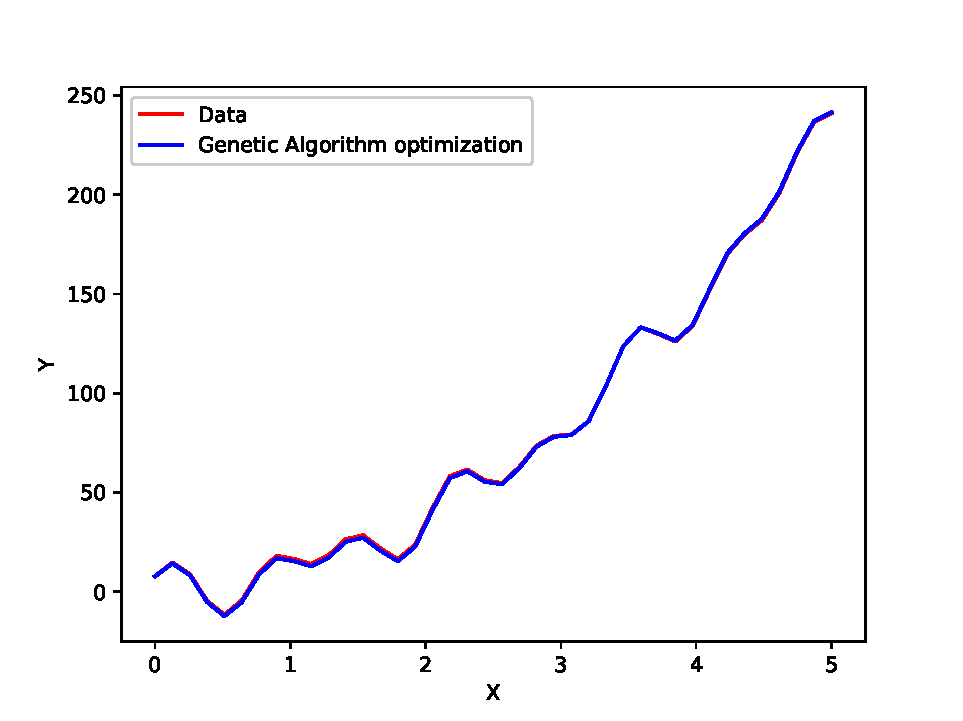
\includegraphics[width=12cm]{../Figure/Q1/Genetic Algorithm_pop_size100_mutation_rate0.5_generations50000_tournament_size20} 
\end{figure}

\begin{figure}[H]
	\caption{جمعیت الگوریتم ژنتیک بر اساس پارامترهای تنظیم شده به صورت \lr{greedy}} 
	\centering 
	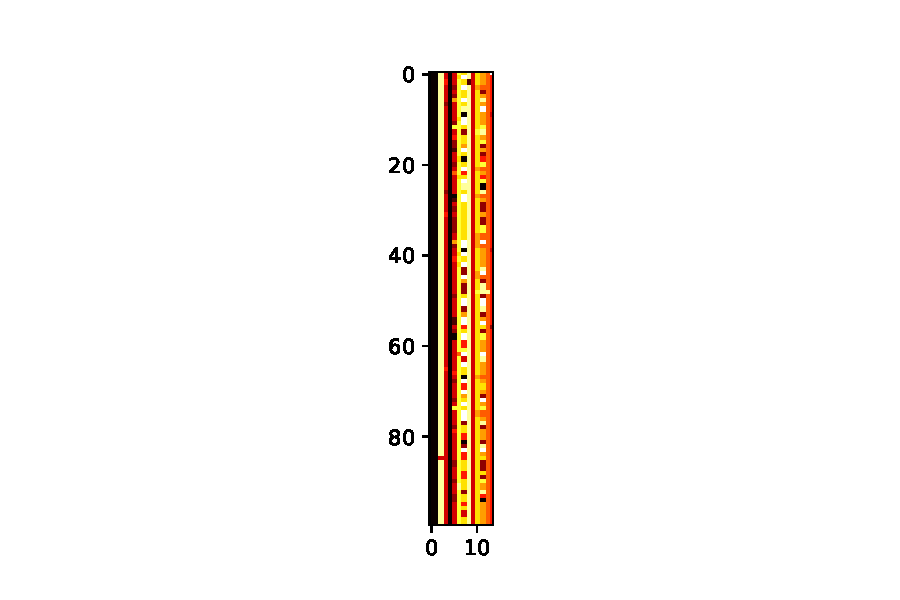
\includegraphics[width=12cm]{../Figure/Q1/Genetic Algorithm_pop_size100_mutation_rate0.5_generations50000_tournament_size20map} 
\end{figure}


\begin{figure}[H]
	\caption{جواب الگوریتم ژنتیک (دودویی) بر اساس پارامترهای تنظیم شده به صورت \lr{greedy}} 
	\centering 
	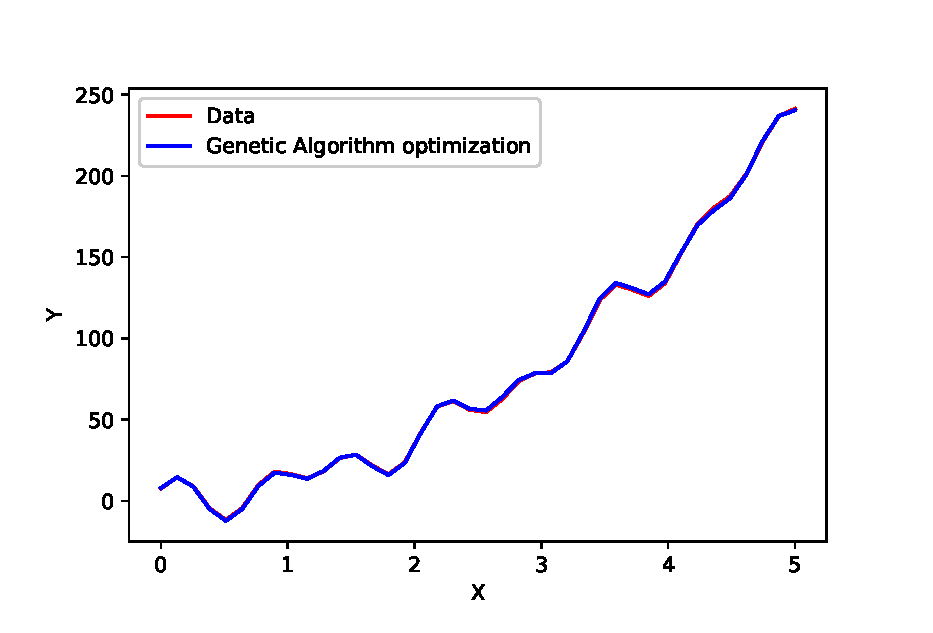
\includegraphics[width=12cm]{../Figure/Q1/Genetic Algorithm_binary_pop_size200_mutation_rate0.5_generations50000_tournament_size50} 
\end{figure}

\begin{figure}[H]
	\caption{جمعیت الگوریتم ژنتیک (دودویی) بر اساس پارامترهای تنظیم شده به صورت \lr{greedy}} 
	\centering 
	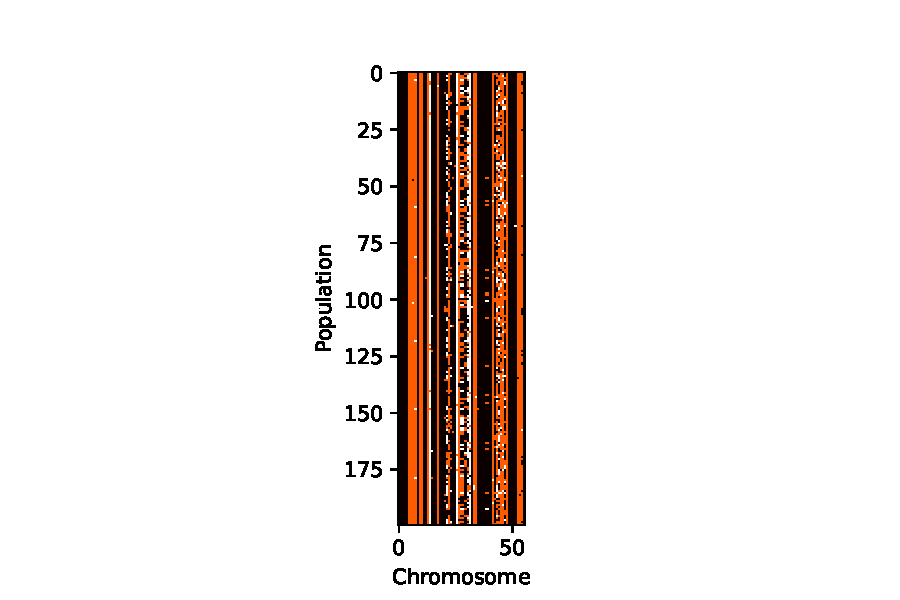
\includegraphics[width=12cm]{../Figure/Q1/Genetic Algorithm_binary_pop_size200_mutation_rate0.5_generations50000_tournament_size50map} 
\end{figure}


\begin{figure}[H]
	\caption{جواب الگوریتم ژنتیک \lr{MATLAB}} 
	\centering 
	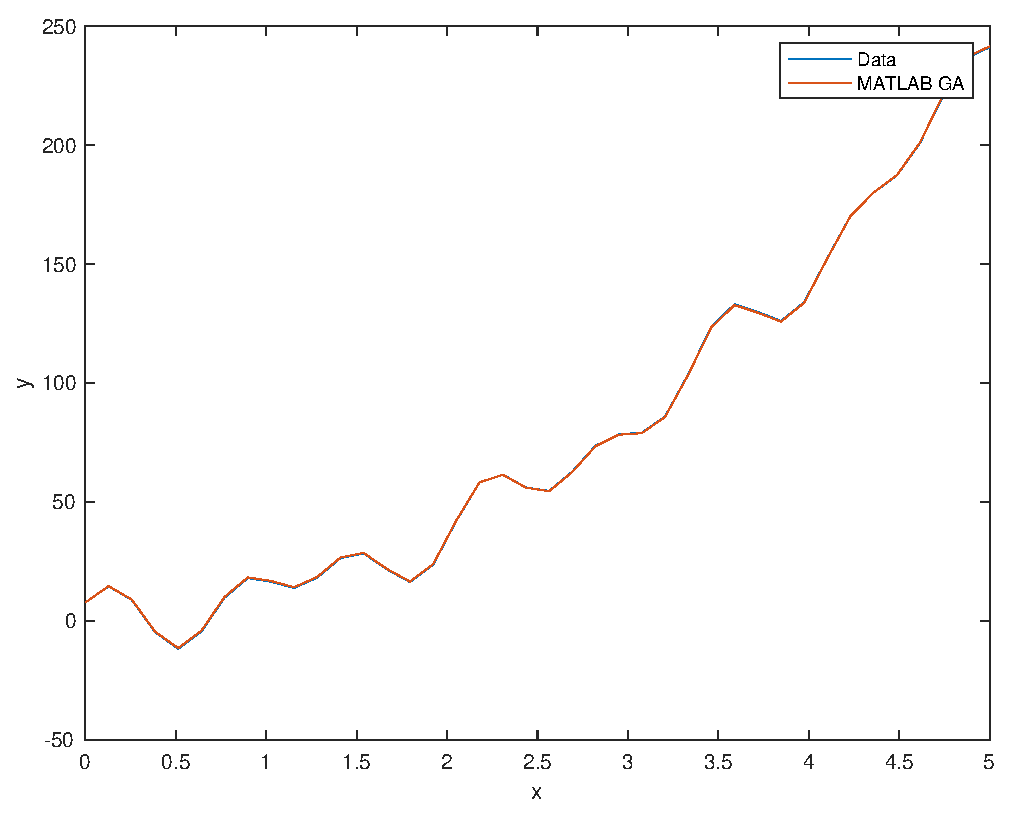
\includegraphics[width=12cm]{../Figure/Q1/MATLAB_GA}
\end{figure}